\documentclass[border=5pt]{standalone}
\usepackage[utf8]{inputenc}
\usepackage[T1]{fontenc}
\usepackage{times}
\usepackage{tikz}
\usetikzlibrary{shapes.geometric, arrows.meta, positioning, calc, shadows.blur, decorations.pathreplacing, backgrounds, fit}

\definecolor{stage1}{HTML}{4472C4}
\definecolor{stage1b}{HTML}{1F6FB5}
\definecolor{stage2}{HTML}{70AD47}
\definecolor{stage3}{HTML}{ED7D31}
\definecolor{epscope}{HTML}{0CA678}
\definecolor{iogray}{HTML}{95A5A6}
\definecolor{titledark}{HTML}{1A3A5C}
\definecolor{databg}{HTML}{F0F0F0}
\definecolor{summbox}{HTML}{FFF3CD}
\definecolor{summbor}{HTML}{FFC107}
\definecolor{epsbg}{HTML}{E6F7EE}
\definecolor{epsbor}{HTML}{0CA678}

\begin{document}
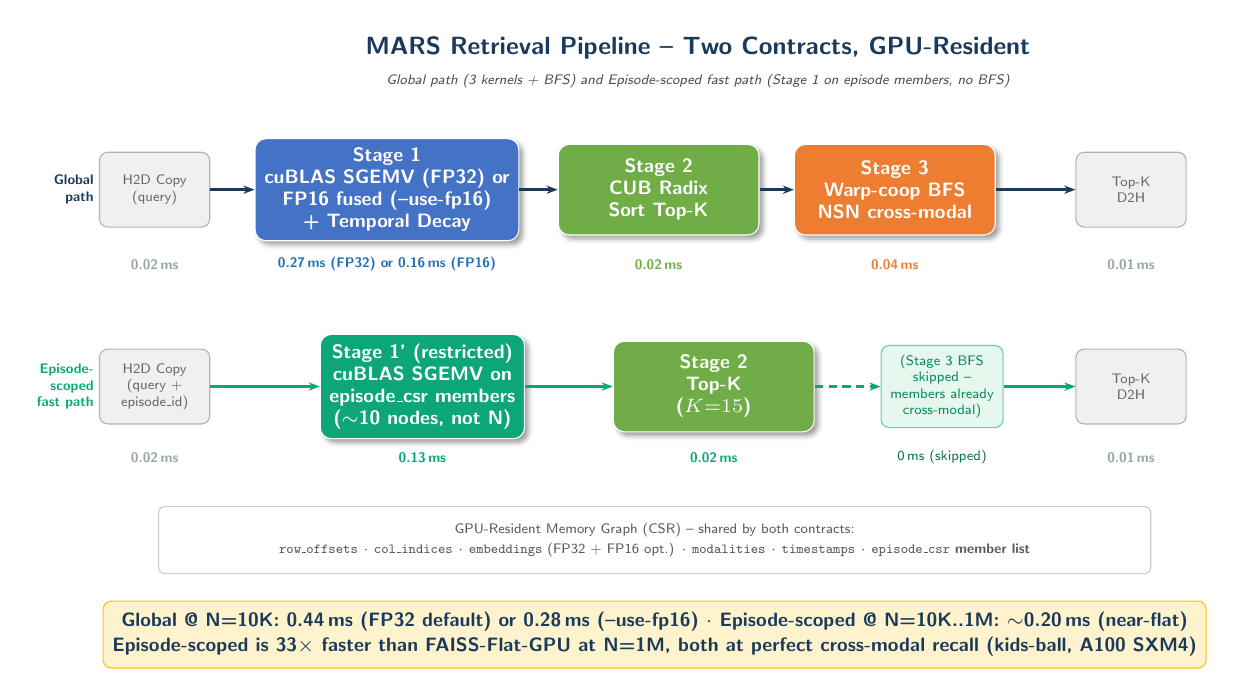
\begin{tikzpicture}[
    stage/.style={draw=white, fill=#1, rounded corners=4pt,
        minimum width=2.55cm, minimum height=1.15cm,
        font=\sffamily\scriptsize\bfseries, text=white, align=center,
        blur shadow={shadow blur steps=3, shadow xshift=0.5mm, shadow yshift=-0.5mm}},
    io/.style={draw=gray!60, fill=databg, rounded corners=3pt,
        minimum width=1.4cm, minimum height=0.95cm,
        font=\sffamily\tiny, text=gray!80!black, align=center},
    datastore/.style={draw=gray!40, fill=white, rounded corners=2pt,
        minimum width=2.4cm, minimum height=0.7cm,
        font=\sffamily\tiny, text=gray!70!black, align=center},
    arr/.style={-{Stealth[length=4pt]}, line width=1.2pt, color=titledark},
    arreps/.style={-{Stealth[length=4pt]}, line width=1.2pt, color=epscope},
    darr/.style={-{Stealth[length=3pt]}, line width=0.7pt, color=gray!50, dashed},
    >=Stealth
]

% ── Title ────────────────────────────────────────────────
\node[font=\sffamily\small\bfseries, text=titledark] at (6.5, 5.6)
    {MARS Retrieval Pipeline -- Two Contracts, GPU-Resident};
\node[font=\sffamily\tiny\itshape, text=gray!60!black] at (6.5, 5.18)
    {Global path (3 kernels + BFS) and Episode-scoped fast path (Stage 1 on episode members, no BFS)};

% ══════════════════════════════════════════════════════════════
% ROW 1 -- GLOBAL PATH (top)
% ══════════════════════════════════════════════════════════════
\node[font=\sffamily\tiny\bfseries, text=titledark, anchor=east, align=right] at (-1.05, 3.8)
    {Global\\path};

\node[io] (input1) at (-0.4, 3.8) {H2D Copy\\(query)};
\node[stage=stage1] (sim1) at (2.55, 3.8) {Stage 1\\cuBLAS SGEMV (FP32) {\itshape or}\\FP16 fused (--use-fp16)\\+ Temporal Decay};
\node[stage=stage2] (topk1) at (6.0, 3.8) {Stage 2\\CUB Radix\\Sort Top-K};
\node[stage=stage3] (bfs1) at (9.0, 3.8) {Stage 3\\Warp-coop BFS\\NSN cross-modal};
\node[io] (output1) at (12.0, 3.8) {Top-K\\D2H};

\draw[arr] (input1.east) -- (sim1.west);
\draw[arr] (sim1.east) -- (topk1.west);
\draw[arr] (topk1.east) -- (bfs1.west);
\draw[arr] (bfs1.east) -- (output1.west);

% Per-stage timings (Global, N=10K, A100 SXM4)
\node[font=\sffamily\tiny\bfseries, text=iogray] at (-0.4, 2.85) {0.02\,ms};
\node[font=\sffamily\tiny\bfseries, text=stage1b] at (2.55, 2.85)
    {0.27\,ms (FP32) {\itshape or} 0.16\,ms (FP16)};
\node[font=\sffamily\tiny\bfseries, text=stage2] at (6.0, 2.85) {0.02\,ms};
\node[font=\sffamily\tiny\bfseries, text=stage3] at (9.0, 2.85) {0.04\,ms};
\node[font=\sffamily\tiny\bfseries, text=iogray] at (12.0, 2.85) {0.01\,ms};

% ══════════════════════════════════════════════════════════════
% ROW 2 -- EPISODE-SCOPED FAST PATH (bottom)
% ══════════════════════════════════════════════════════════════
\node[font=\sffamily\tiny\bfseries, text=epscope, anchor=east, align=right] at (-1.05, 1.30)
    {Episode-\\scoped\\fast path};

\node[io] (input2) at (-0.4, 1.30) {H2D Copy\\(query +\\episode\_id)};
\node[stage=epscope] (sim2) at (3.0, 1.30) {Stage 1' (restricted)\\cuBLAS SGEMV on\\episode\_csr members\\($\sim$10 nodes, not N)};
\node[stage=stage2] (topk2) at (6.7, 1.30) {Stage 2\\Top-K\\($K{=}15$)};
\node[io, draw=epsbor!60, fill=epsbg, text=epscope!80!black] (output2) at (9.6, 1.30)
    {(Stage 3 BFS\\skipped --\\members already\\cross-modal)};
\node[io] (output2b) at (12.0, 1.30) {Top-K\\D2H};

\draw[arreps] (input2.east) -- (sim2.west);
\draw[arreps] (sim2.east) -- (topk2.west);
\draw[arreps, densely dashed] (topk2.east) -- (output2.west);
\draw[arreps] (output2.east) -- (output2b.west);

% Per-stage timings (Episode-scoped, any N)
\node[font=\sffamily\tiny\bfseries, text=iogray] at (-0.4, 0.40) {0.02\,ms};
\node[font=\sffamily\tiny\bfseries, text=epscope] at (3.0, 0.40) {0.13\,ms};
\node[font=\sffamily\tiny\bfseries, text=epscope] at (6.7, 0.40) {0.02\,ms};
\node[font=\sffamily\tiny, text=epscope!70!black] at (9.6, 0.40) {0\,ms (skipped)};
\node[font=\sffamily\tiny\bfseries, text=iogray] at (12.0, 0.40) {0.01\,ms};

% ── GPU-Resident Memory Graph (shared between contracts) ────
\node[draw=gray!40, fill=white, rounded corners=2pt,
      minimum width=12.6cm, minimum height=0.85cm,
      font=\sffamily\tiny, text=gray!70!black, align=center]
      (graph) at (5.95, -0.65)
      {GPU-Resident Memory Graph (CSR) -- shared by both contracts:\\[1pt]
       \texttt{row\_offsets} $\cdot$ \texttt{col\_indices} $\cdot$ \texttt{embeddings} (FP32 + FP16 opt.) $\cdot$ \texttt{modalities} $\cdot$ \texttt{timestamps} $\cdot$ \textbf{\texttt{episode\_csr} member list}};

% ── Summary box ──────────────────────────────────────────
\node[draw=summbor, fill=summbox, rounded corners=3pt,
      font=\sffamily\scriptsize\bfseries, text=titledark,
      minimum width=12.6cm, minimum height=0.85cm, align=center]
      at (5.95, -1.85)
      {Global @ N=10K: \textbf{0.44\,ms} (FP32 default) {\itshape or} \textbf{0.28\,ms} (--use-fp16)
        $\cdot$ Episode-scoped @ N=10K..1M: \textbf{$\sim$0.20\,ms (near-flat)}\\[1pt]
       Episode-scoped is 33$\times$ faster than FAISS-Flat-GPU at N=1M, both at perfect cross-modal recall (kids-ball, A100 SXM4)};

\end{tikzpicture}
\end{document}
